\section{Mockups}
A propósito de desenhar um design para seguir e apresentar às partes interessadas antes de iniciar a 
fase de desenvolvimento, então foram realizadas mockups do design da aplicação. Este design foi 
iterativamente revisto pelas partes interessadas e afinado até chegar ao seu estado final.

\subsection{Página Inicial}

A página inicial da aplicação, dá ao utilizador a possibilidade de navegar pelo produtos do catálogo,
conseguindo também filtrar pelas categorias e subcategorias do catálogo, 
assim como também realizar uma pesquisa rápida pelos produtos, por fim este poderá navegar para o fórum.
Caso um técnico esteja com sessão iniciada este poderá também visualizar o icon de notificações e a sua 
imagem de perfil.

\begin{figure}[htb]
    \centering
    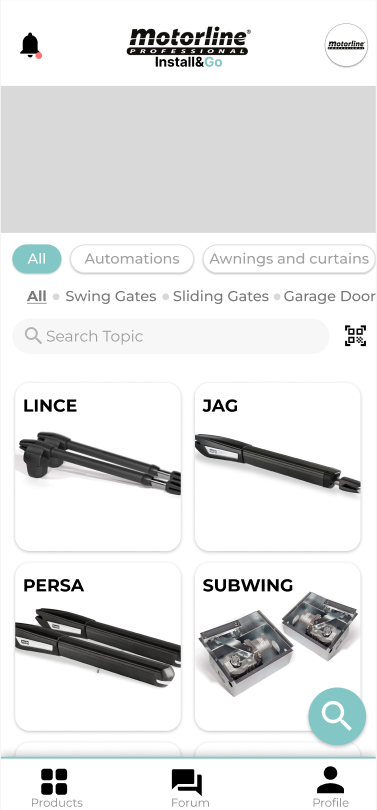
\includegraphics[width=0.4\textwidth]{images/mockups/home_screen.png}
    \caption{Página inicial do fórum}
    \label{fig:16}
\end{figure}

\newpage

\subsection{Autenticação - Login e Registo}

Na autenticação primeiramente é possivel realizar o login, onde o técnico poderá iniciar sessão no software 
e registo onde a empresa poderá realizar o registo no software.

\begin{figure}[htb]%
    \centering
    \subfloat[\centering Página de login]{{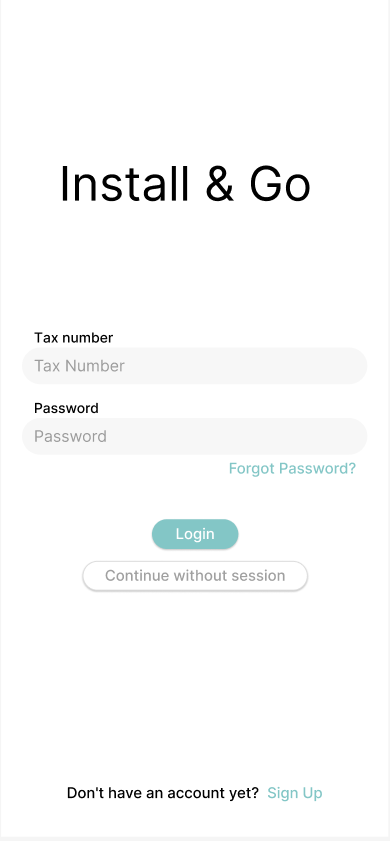
\includegraphics[width=0.4\textwidth]{images/mockups/login.png} }}%
    \qquad
    \subfloat[\centering Página de registo]{{
\includegraphics[width=0.4\textwidth]{images/mockups/register.png} }}%
    \caption{Autenticação - Login e Registo}%
    \label{fig:17}%
\end{figure}

\newpage

\subsection{Autenticação - Ativação e Confirmação de conta}

Na autenticação tem existe a página de confirmação de conta, onde um técnico que tem a sua conta recentemente adicionada poderá
confirmar o registo da conta indicando as informações finais de conta, sendo por fim direcionado para a página
de ativação de conta onde terá de colocar o código de ativação enviado para o seu email, esta página será também aberta 
caso um técnico realize login com uma conta que não foi ativada ou então sempre que um registo é finalizado.

\begin{figure}[htb]%
    \centering
    \subfloat[\centering Página de confirmação de conta]{{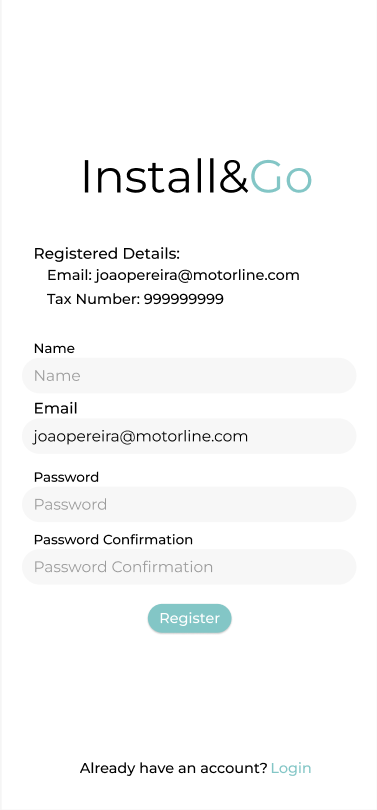
\includegraphics[width=0.4\textwidth]{images/mockups/account_confirmation.png} }}%
    \qquad
    \subfloat[\centering Página de ativação de conta]{{
\includegraphics[width=0.4\textwidth]{images/mockups/account_verification.png} }}%
    \caption{Autenticação - Ativação e Confirmação de conta}%
    \label{fig:17}%
\end{figure}

\newpage

\subsection{Página inicial fórum}

O utilizador assim que se dirige ao fórum entrará na página inicial do mesmo, esta página permite navegar 
entre as diferentes listagens de tópicos acessíveis ao utilizador, aceder à página de pesquisas, filtrar a 
listagem atual por tipo de tópico e caso um técnico entre nesta página ele poderá também criar um novo 
tópico.

\begin{figure}[htb]
    \centering
    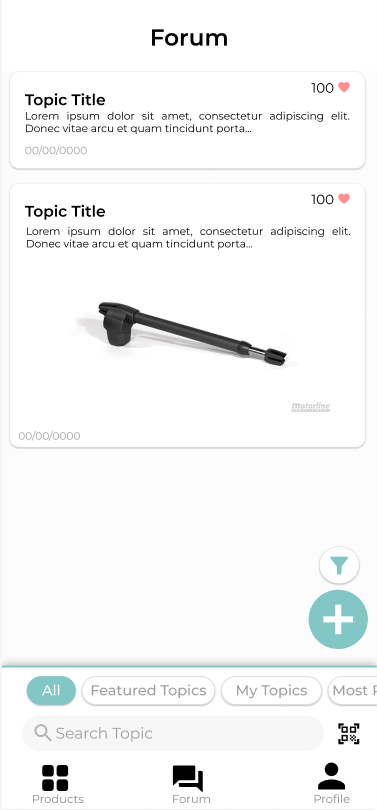
\includegraphics[width=0.5\textwidth]{images/mockups/forum_home.png}
    \caption{Página inicial do fórum}
    \label{fig:18}
\end{figure}

\newpage

\subsection{Página de detalhes de um tópico}

Assim que o utilizador seleciona um tópico ele será encaminhado para a página de detalhes de um tópico, onde 
é indicado o nome do dono do tópico, a sua imagem de perfil, a hora de criação do mesmo, a quantidade de 
gostos, o título, descrição, imagens e comentários do tópico. Nesta página o utilizador poderá visualizar 
todas as respostas. 
Por fim o técnico consegue, além disso, gostar do tópico, gostar de respostas, responder ao tópico e a outras respostas.

Se o tópico for do técnico que está a visualizar o mesmo, este poderá também concluir, eliminar o tópico e alterar 
a sua visibilidade.

\begin{figure}[htb]%
    \centering
    \subfloat[\centering Página de detalhes de um tópico]{{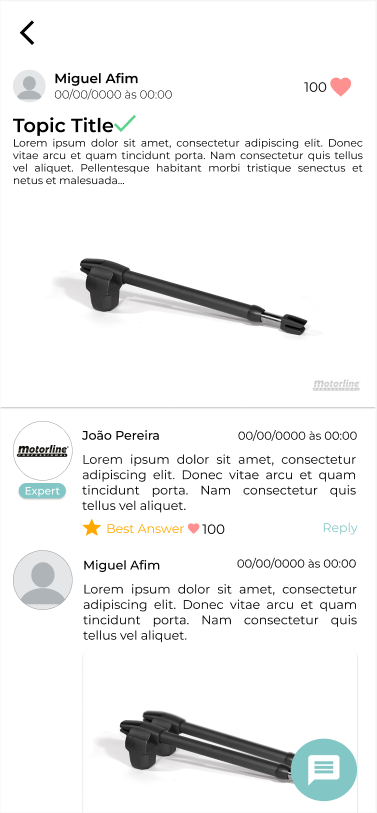
\includegraphics[width=0.4\textwidth]{images/mockups/topic_not_user.png} }}%
    \qquad
    \subfloat[\centering Página de detalhes de um tópico do técnico]{{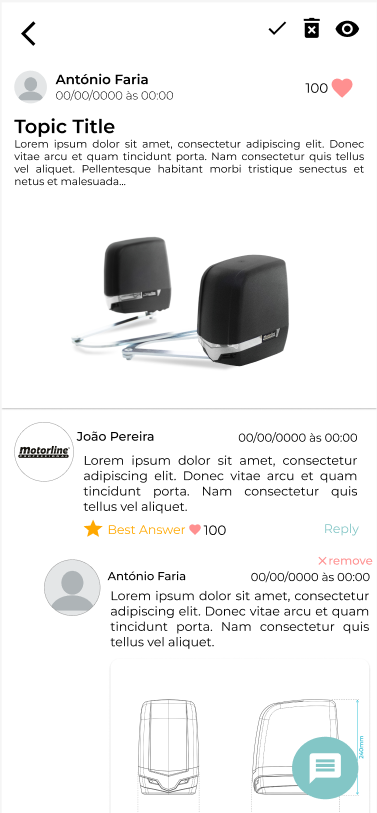
\includegraphics[width=0.4\textwidth]{images/mockups/user_topic.png} }}%
    \caption{Página de detalhes de tópico do software}%
    \label{fig:20}%
\end{figure}

\newpage

\subsection{Página de criação de um tópico}

Quando um técnico inicia a criação de um tópico, este será direcionado para a página de criação de tópico, 
nesta página o técnico poderá inserir o título e descrição do tópico, assim como indicar a visibilidade do 
tópico, o tipo de tópico, o produto referente e por fim o técnico poderá anexar imagens. 
A qualquer momento o técnico poderá cancelar ou confirmar a criação do tópico.

\begin{figure}[htb]
    \centering
    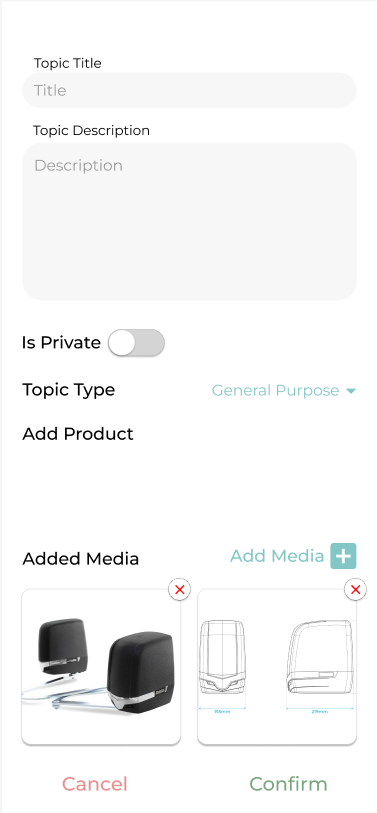
\includegraphics[width=0.5\textwidth]{images/mockups/forum_create_topic.png}
    \caption{Página de criação de tópico}
    \label{fig:21}
\end{figure}

\subsection{Página de notificações}

Um técnico sempre que desejar poderá visualizar as suas notificações, para isso deverá se dirigir à página
de notificações, neste é possível ver todas as notificações identificando quem enviou, qual a descrição da 
notificação e data de receção desta. O técnico poderá também apagar a notificação se assim desejar.

\begin{figure}[htb]
    \centering
    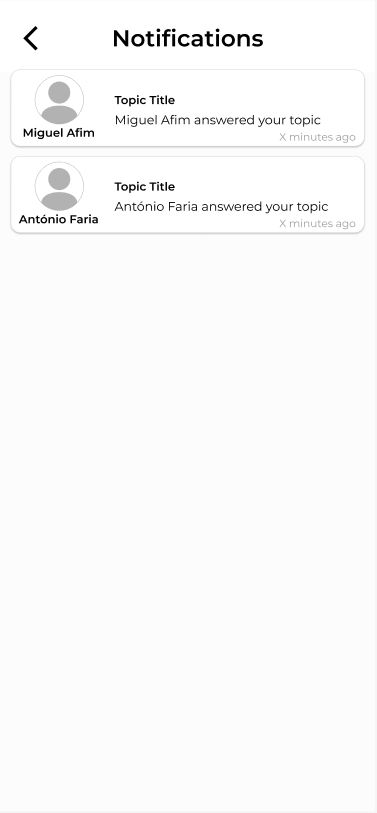
\includegraphics[width=0.5\textwidth]{images/mockups/notifications.png}
    \caption{Página de notificações}
    \label{fig:22}
\end{figure}

\newpage

\subsection{Página de perfil de utilizador}

O técnico sempre que desejar alterar as suas informações, deverá se deslocar ao seu perfil no qual é possível
alterar o se nome, email e imagem de perfil. Neste é possível também configurar as notificações indicando os métodos
a receber notificação e o tipo de notificação a receber para cada método selecionado.

Caso uma empresa entre no perfil esta visualizará um botão para aceder à gestão de recursos humanos.

\begin{figure}[htb]
    \centering
    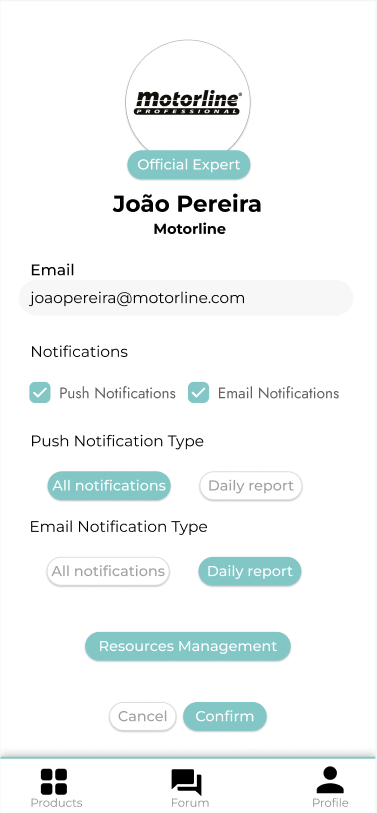
\includegraphics[width=0.5\textwidth]{images/mockups/user_profile.png}
    \caption{Página de perfil de utilizador}
    \label{fig:23}
\end{figure}

\subsection{Página de gestão de recursos humanos}

Sempre que é necessário registar novas contas de técnico a empresa deverá direcionar-se à página de gestão
de recursos humanos, nesta página esta poderá registar novos técnicos ou gerir os técnicos já registados,
conseguindo aceder aos seus perfis. Por fim a empresa consegue também pesquisar por técnico.

\begin{figure}[htb]
    \centering
    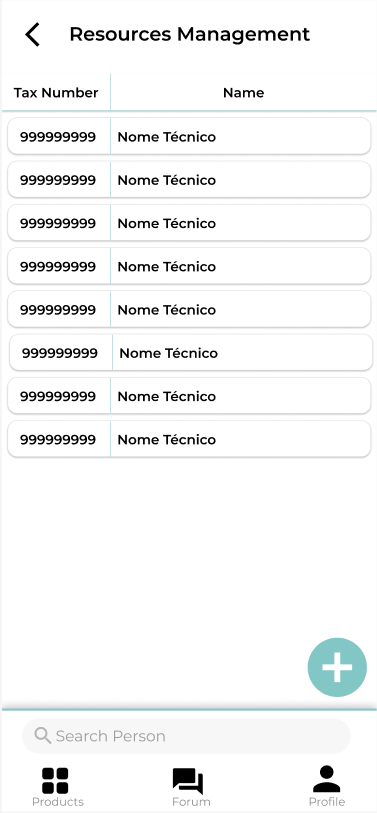
\includegraphics[width=0.5\textwidth]{images/mockups/human_resources.png}
    \caption{Página de gestão de recursos humanos}
    \label{fig:24}
\end{figure}

\newpage

\subsection{Página de perfil de técnico registado}

Para ver as estatisticas de um técnico ou para realizar alguma operação sobre este, a empresa deverá
clicar no técnico desejado na página de recursos humanos, onde será direcionada para a página de perfil do
técnico e visualizará as estatisticas deste, assim como também as suas informações e tem a possibilidade
de impedir acesso à conta ou então remover a conta da plataforma.

\begin{figure}[htb]
    \centering
    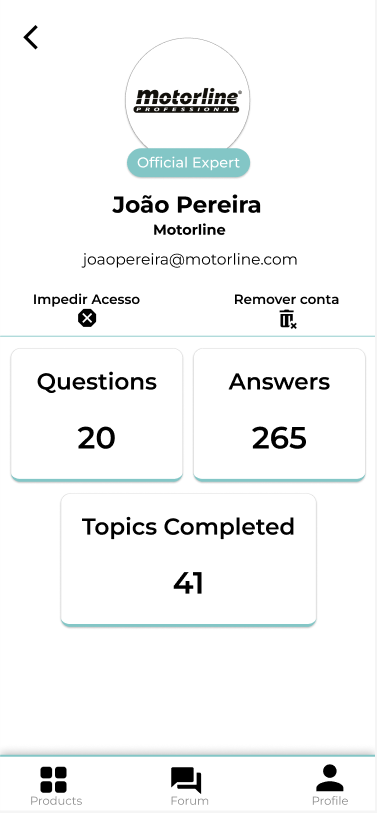
\includegraphics[width=0.5\textwidth]{images/mockups/professional_profile.png}
    \caption{Página de perfil de técnico registado}
    \label{fig:24}
\end{figure}

\subsection{Página de registo de novo técnico}

Sempre que uma empresa deseja registar um novo técnico esta deverá clicar em registar novo técnico onde será
direcionada para a página de registo de técnicos, nesta página é pedido o número de contribuinte e email do 
técnico.

\begin{figure}[htb]
    \centering
    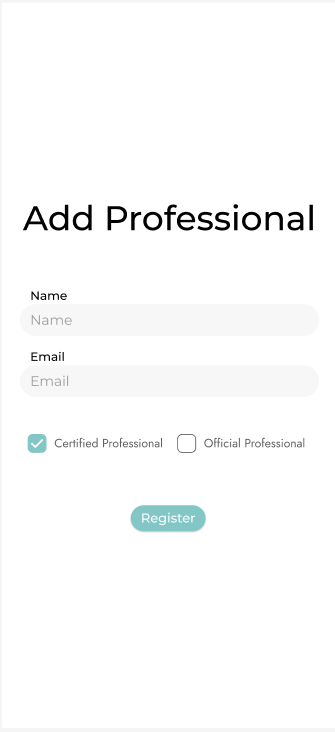
\includegraphics[width=0.5\textwidth]{images/mockups/account_registering.png}
    \caption{Página de registo de novo técnico}
    \label{fig:24}
\end{figure}